\documentclass{article}

% content/resources/templates/preamble.tex
\usepackage[margin=0.6in]{geometry}
\author{Milav Dabgar}
\usepackage{amsmath,amssymb,amsthm}
\usepackage{booktabs}
\usepackage{multirow}
\usepackage{xcolor}
\usepackage{tcolorbox}
\tcbuselibrary{breakable,skins}
\usepackage[colorlinks=true,linkcolor=blue]{hyperref}
\usepackage{titlesec}
\usepackage{enumitem}
\usepackage{tikz}
\usepackage{pgfplots}
\usepackage{circuitikz}
\usepackage[version=4]{mhchem}
\usepackage{longtable}
\usepackage{array}
\usepackage{float}
\usepackage{caption}
\usepackage{listings}

\lstset{
  basicstyle=\small\ttfamily,
  breaklines=true,
  breakatwhitespace=false,
  postbreak=\mbox{\textcolor{red}{$\hookrightarrow$}\space},
  float=false,
  numbers=left,
  numberstyle=\tiny\color{gray},
  numbersep=10pt,
  xleftmargin=2em,
  keywordstyle=\color{blue},
  commentstyle=\color{green!60!black},
  stringstyle=\color{purple},
  backgroundcolor=\color{gray!5},
  showstringspaces=false,
  tabsize=2,
  captionpos=b,
  keepspaces=true,
  columns=flexible
}

\pgfplotsset{compat=1.18}
\usetikzlibrary{shapes,arrows,positioning,calc,patterns,decorations.pathmorphing,decorations.markings,arrows.meta}

% Color scheme
\definecolor{headcolor}{RGB}{0,102,204}
\definecolor{keycolor}{RGB}{220,20,60}
\definecolor{solutioncolor}{RGB}{34,139,34}
\definecolor{mnemoniccolor}{RGB}{148,0,211}
\definecolor{codecolor}{RGB}{0,0,100}

% Spacing
\setlength{\parskip}{3pt}
\setlist[itemize]{nosep}
\setlist[enumerate]{nosep}

% Title formatting
\titleformat{\section}{\Large\bfseries\color{headcolor}}{\thesection}{1em}{}
\titleformat{\subsection}{\large\bfseries\color{headcolor}}{\thesubsection}{1em}{}

% Pandoc tightlist compatibility
\providecommand{\tightlist}{%
  \setlength{\itemsep}{0pt}\setlength{\parskip}{0pt}}

% Pandoc longtable compatibility
\newcounter{none}
\def\thenone{}


\title{Fundamentals of Electronics (DI01000051) - Summer 2025 Solution}
\date{June 12, 2025}

% PDF Metadata
\hypersetup{
  pdftitle={Fundamentals of Electronics (DI01000051) - Summer 2025 Solution},
  pdfsubject={GTU Exam Solution - Summer-2025},
  pdfauthor={Milav Dabgar},
  pdfkeywords={DI01000051, Electronics, Fundamentals, Summer 2025, GTU, Solution},
  pdfcreator={XeLaTeX}
}

\begin{document}
\maketitle

\setcounter{tocdepth}{5}
\tableofcontents
\newpage

% ========================================
% QUESTION 1
% ========================================
\section{Question 1}

\subsection{Question 1(a) [3 marks]}
\textbf{Draw Bi-stable multivibrator using 555 timer IC.}

\subsubsection{Solution}
A **Bi-stable multivibrator** has two stable states (High and Low). It remains in one state until triggered to switch to the other.

\paragraph{Circuit Diagram:}
\begin{figure}[H]
\centering
\begin{circuitikz}[scale=1.0]
    \draw (0,0) node[dipchip, num pins=8, hide numbers, external pins width=0, anchor=center] (U1) {555};
    % Label pins
    \node [right, font=\tiny] at (U1.bpin 1) {GND};
    \node [right, font=\tiny] at (U1.bpin 2) {TRIG};
    \node [right, font=\tiny] at (U1.bpin 3) {OUT};
    \node [right, font=\tiny] at (U1.bpin 4) {RST};
    \node [left, font=\tiny] at (U1.bpin 8) {VCC};
    \node [left, font=\tiny] at (U1.bpin 6) {THR};
    \node [left, font=\tiny] at (U1.bpin 5) {CV};
    \node [left, font=\tiny] at (U1.bpin 7) {DIS};

    % Connections
    \draw (U1.bpin 1) -- ++(0,-0.5) node[ground]{};
    \draw (U1.bpin 8) -- ++(0,0.5) node[vcc]{VCC};
    
    % Trigger switch
    \draw (U1.bpin 2) -- ++(-1,0) to[push button, l=Set] ++(0,-1) node[ground]{};
    \draw (U1.bpin 2) ++(-1,0) to[R, l=10k] ++(0,2) node[vcc]{VCC};

    % Reset switch
    \draw (U1.bpin 4) -- ++(-2,0) to[push button, l=Reset] ++(0,-1.75) node[ground]{};
    \draw (U1.bpin 4) ++(-2,0) to[R, l=10k] ++(0,2) node[vcc]{VCC};
    
    % Threshold grounded
    \draw (U1.bpin 6) -- ++(2,0) node[ground]{};
    
    % Output LED
    \draw (U1.bpin 3) -- ++(1,0) to[R, l=330] ++(2,0) to[leDo] ++(0,-1.5) node[ground]{};

\end{circuitikz}
\caption{Bi-stable Multivibrator using 555 Timer}
\end{figure}

\paragraph{Working:}
\begin{itemize}
    \item When **Trigger (Pin 2)** is pressed (Low), Output goes **HIGH**.
    \item When **Reset (Pin 4)** is pressed (Low), Output goes **LOW**.
    \item Threshold (Pin 6) is grounded to preventing accidental switching.
\end{itemize}

\paragraph{Mnemonic:}
\emph{Bi-Stable: Two Switches, Two States (Set \& Reset).}

\subsection{Question 1(b) [4 marks]}
\textbf{Draw pin diagram of IC 555 timer and explain it.}

\subsubsection{Solution}

\paragraph{Pin Diagram:}
\begin{figure}[H]
\centering
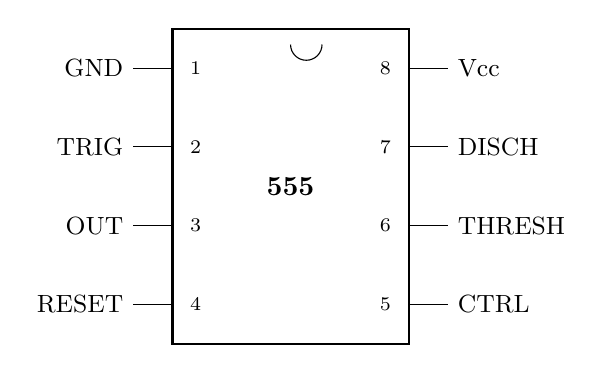
\begin{tikzpicture}
    % Body
    \draw[thick] (0,0) rectangle (3,4);
    \node at (1.5,2) {\textbf{555}};
    \draw (1.5,3.8) arc (180:360:0.2); % Notch
    
    % Pins Left
    \foreach \i/\label in {1/GND, 2/TRIG, 3/OUT, 4/RESET} {
        \draw (0, 4.5-\i) -- (-0.5, 4.5-\i);
        \node[right] at (0.1, 4.5-\i) {\scriptsize \i};
        \node[left] at (-0.5, 4.5-\i) {\small \label};
    }
    
    % Pins Right
    \foreach \i/\label in {8/Vcc, 7/DISCH, 6/THRESH, 5/CTRL} {
        \draw (3, \i-4.5) -- (3.5, \i-4.5);
        \node[left] at (2.9, \i-4.5) {\scriptsize \i};
        \node[right] at (3.5, \i-4.5) {\small \label};
    }
\end{tikzpicture}
\caption{Pin Configuration of 555 Timer}
\end{figure}

\paragraph{Pin Description:}
\begin{description}
    \item[Pin 1 (GND):] Ground reference voltage (0V).
    \item[Pin 2 (Trigger):] Turns output HIGH when voltage drops below 1/3 Vcc.
    \item[Pin 3 (Output):] Output signal (sourcing/sinking max 200mA).
    \item[Pin 4 (Reset):] Resets the timer when grounded (active low).
    \item[Pin 5 (Control Voltage):] Access to internal voltage divider (2/3 Vcc).
    \item[Pin 6 (Threshold):] Turns output LOW when voltage exceeds 2/3 Vcc.
    \item[Pin 7 (Discharge):] Provides discharge path for external capacitor.
    \item[Pin 8 (Vcc):] Supply voltage (+5V to +18V).
\end{description}

\paragraph{Mnemonic:}
\emph{GTOR CV T D V: Ground, Trigger, Output, Reset | Control, Threshold, Discharge, Vcc.}

\subsection{Question 1(c) [7 marks]}
\textbf{Draw and Explain block diagram of IC 555 timer.}

\subsubsection{Solution}

\paragraph{Block Diagram:}
\begin{figure}[H]
\centering
\begin{tikzpicture}[scale=0.8, transform shape]
    % Resistors Divider
    \draw (2,8) node[vcc]{Vcc} to[R, l=5k] (2,6) to[R, l=5k] (2,4) to[R, l=5k] (2,2) node[ground]{};
    
    % Comparators
    \draw (5,6) node[op amp, anchor=minus] (C1) {};
    \draw (5,3) node[op amp, anchor=plus] (C2) {};
    \node at (C1) {Comp A};
    \node at (C2) {Comp B};
    
    % Connections to Comparators
    \draw (2,6) -- (C1.minus);
    \draw (2,2.67) -| (C2.plus);
    
    % Inputs
    \draw (C1.plus) -- ++(-1,0) node[left] {Threshold (6)};
    \draw (C2.minus) -- ++(-1,0) node[left] {Trigger (2)};
    
    % Flip Flop
    \draw (8,4.5) node[draw, minimum width=2cm, minimum height=3cm] (FF) {SR Flip-Flop};
    \node at (7.5, 5.5) {R};
    \node at (7.5, 3.5) {S};
    \node at (8.5, 5.5) {Q};
    \node at (8.5, 3.5) {\(\bar{Q}\)};
    
    % Connections to FF
    \draw (C1.out) -- (7,6) -- (7,5.5) -- (FF.west |- 0,5.5);
    \draw (C2.out) -- (7,3) -- (7,3.5) -- (FF.west |- 0,3.5);
    
    % Output Stage
    \draw (FF.east |- 0,3.5) -- ++(1,0) node[draw] (NOT) {NOT} -- ++(1,0) node[right] {Output (3)};
    
    % Discharge Transistor
    \draw (FF.east |- 0,5.5) -- ++(0.5,0) -- ++(0,1) node[npn, anchor=B] (Q1) {};
    \draw (Q1.C) -- ++(0,0.5) node[above] {Discharge (7)};
    \draw (Q1.E) node[ground]{};

    % Reset
    \draw (8, 6.5) node[above] {Reset (4)} -- (FF.north);
    
    % Control Voltage
    \draw (2,6) -- ++(-1,0) node[left] {Control (5)};

\end{tikzpicture}
\caption{Internal Block Diagram of 555 Timer}
\end{figure}

\paragraph{Explanation:}
The 555 timer consists of:
\begin{enumerate}
    \item \textbf{Voltage Divider:} Three 5k\(\Omega\) resistors divide Vcc into 1/3 Vcc and 2/3 Vcc reference voltages.
    \item \textbf{Comparators:}
        \begin{itemize}
            \item **Comparator A (Upper):** Compares Threshold (Pin 6) with 2/3 Vcc. If Pin 6 > 2/3 Vcc, Output is High (Resets FF).
            \item **Comparator B (Lower):** Compares Trigger (Pin 2) with 1/3 Vcc. If Pin 2 < 1/3 Vcc, Output is High (Sets FF).
        \end{itemize}
    \item \textbf{RS Flip-Flop:} Stores the state. Set by Trigger, Reset by Threshold.
    \item \textbf{Output Driver:} Inverts \(\bar{Q}\) output to drive the load (Pin 3).
    \item \textbf{Discharge Transistor:} Discharges external capacitor when proper logic is met (Pin 7).
\end{enumerate}

\paragraph{Mnemonic:}
\emph{3-5-2-1: 3 Resistors, 5-5-5, 2 Comparators, 1 Flip-Flop.}

\subsection*{OR}

\subsection{Question 1(c) [7 marks]}
\textbf{Draw and Explain A-stable and mono-stable multivibrator using 555 timer IC.}

\subsubsection{Solution}

\paragraph{1. Astable Multivibrator (Free Running):}
Generates a continuous square wave without external triggering.

\textbf{Circuit Diagram:}
\begin{figure}[H]
\centering
\begin{circuitikz}[scale=0.8]
    \draw (0,0) node[dipchip, num pins=8, hide numbers, external pins width=0, anchor=center] (U1) {555};
    % VCC and Ground
    \draw (U1.bpin 8) -- ++(0,0.5) node[vcc]{Vcc};
    \draw (U1.bpin 1) -- ++(0,-0.5) node[ground]{};
    % Connections
    \draw (U1.bpin 4) -- (U1.bpin 8); % Reset to Vcc
    \draw (U1.bpin 2) -- (U1.bpin 6); % Trigger connected to Threshold
    \draw (U1.bpin 7) to[R, l=\(R_A\)] (U1.bpin 8);
    \draw (U1.bpin 7) to[R, l=\(R_B\)] (U1.bpin 6);
    \draw (U1.bpin 6) to[C, l=\(C\)] ++(0,-2) node[ground]{};
    \draw (U1.bpin 3) -- ++(1,0) node[right]{Output};
\end{circuitikz}
\end{figure}

\begin{itemize}
    \item **Operation:** Capacitor C charges through \(R_A + R_B\) to 2/3 Vcc, then discharges through \(R_B\) to 1/3 Vcc.
    \item **Output:** Cycles between High and Low continuously.
\end{itemize}

\paragraph{2. Monostable Multivibrator (One Shot):}
Produces a single output pulse of fixed duration when triggered.

\textbf{Circuit Diagram:}
\begin{figure}[H]
\centering
\begin{circuitikz}[scale=0.8]
    \draw (0,0) node[dipchip, num pins=8, hide numbers, external pins width=0, anchor=center] (U1) {555};
    % VCC and Ground
    \draw (U1.bpin 8) -- ++(0,0.5) node[vcc]{Vcc};
    \draw (U1.bpin 1) -- ++(0,-0.5) node[ground]{};
    % Connections
    \draw (U1.bpin 4) -- (U1.bpin 8); % Reset to Vcc
    \draw (U1.bpin 6) -- (U1.bpin 7); % Threshold connected to Discharge
    \draw (U1.bpin 8) to[R, l=\(R\)] (U1.bpin 7);
    \draw (U1.bpin 7) to[C, l=\(C\)] ++(0,-2) node[ground]{};
    \draw (U1.bpin 2) to[short,-o] ++(-1,0) node[left]{Trig};
    \draw (U1.bpin 3) -- ++(1,0) node[right]{Output};
\end{circuitikz}
\end{figure}

\begin{itemize}
    \item **Operation:** When triggered, output goes High. C charges through R. When \(V_c = 2/3 Vcc\), output goes Low.
    \item **Pulse Width:** \(T = 1.1 RC\).
\end{itemize}

\paragraph{Mnemonic:}
\emph{Astable = Infinite loops (Free running). Monostable = One pulse (One shot).}

% ========================================
% QUESTION 2
% ========================================
\section{Question 2}

\subsection{Question 2(a) [3 marks]}
\textbf{Write short note on Active components and passive components.}

\subsubsection{Solution}

\paragraph{Comparison:}
\begin{description}
    \item[Active Components:] Components that **can amplify** an electrical signal or produce power gain. They require an external source to operate.
        \begin{itemize}
            \item **Examples:** Transistors (BJT, FET), Diodes, Op-Amps, SCR.
            \item **Function:** Switching, Amplification, Regulation.
        \end{itemize}
    \item[Passive Components:] Components that **cannot amplify** a signal. They dissipate or store energy.
        \begin{itemize}
            \item **Examples:** Resistors, Capacitors, Inductors, Transformers.
            \item **Function:** Attenuation, Energy Storage, Filtering.
        \end{itemize}
\end{description}

\paragraph{Mnemonic:}
\emph{Active Acts (Controls/Amplifies), Passive Passes (Consumes/Stores).}

\subsection{Question 2(b) [4 marks]}
\textbf{Write color band of following resistance. (1) 47 \(\Omega \pm 5\%\)}

\subsubsection{Solution}
To find the color code for \(47\,\Omega \pm 5\%\):

\paragraph{Calculation:}
\begin{itemize}
    \item **1st Digit (4):** Yellow
    \item **2nd Digit (7):** Violet
    \item **Multiplier (\(10^0 = 1\)):** Black (\(47 \times 1 = 47\))
    \item **Tolerance (\(\pm 5\%\)):** Gold
\end{itemize}

\paragraph{Result:}
**Yellow - Violet - Black - Gold**

\paragraph{Mnemonic:}
\emph{BBROYGBVGW -> Black(0) Brown(1) Red(2) Orange(3) Yellow(4) Green(5) Blue(6) Violet(7) Grey(8) White(9).}

\subsection{Question 2(c) [7 marks]}
\textbf{Explain working of Full wave center tap rectifier with circuit diagram and wave form.}

\subsubsection{Solution}

\paragraph{Circuit Diagram:}
\begin{figure}[H]
\centering
\begin{circuitikz}[scale=1.0]
    \draw (0,3) to[sV, l=\(V_{in}\)] (0,0);
    \draw (0,3) -- (1,3);
    \draw (0,0) -- (1,0);
    % Transformer
    \draw (1,0) node[transformer core](T){} (1,3);
    \draw (T.B1) -- (3.5, 3) to[D, l=\(D_1\)] (5.5,3) -- (6,3);
    \draw (T.B2) -- (3.5, 0) to[D, l=\(D_2\)] (5.5,0) -- (6,0);
    \draw (6,3) -- (6,0); % Short D1 and D2 cathodes
    \draw (6,1.5) to[short, *-] (7,1.5) to[R, l=\(R_L\)] (7,-1.5) node[ground]{};
    % Center Tap
    \draw (T.base) to[short, *-] (2.7, 1.5) |- (7,-1.5); % Connect CT to Ground
\end{circuitikz}
\caption{Full Wave Center Tap Rectifier}
\end{figure}

\paragraph{Working:}
\begin{itemize}
    \item A center-tap transformer with two diodes (\(D_1, D_2\)) is used.
    \item **Positive Half Cycle:** \(D_1\) is forward biased (Conducts), \(D_2\) is reverse biased. Current flows through \(D_1\) and Load.
    \item **Negative Half Cycle:** \(D_2\) is forward biased (Conducts), \(D_1\) is reverse biased. Current flows through \(D_2\) and Load.
    \item Current direction in \(R_L\) remains same for both cycles.
\end{itemize}

\paragraph{Waveforms:}
\begin{figure}[H]
\centering
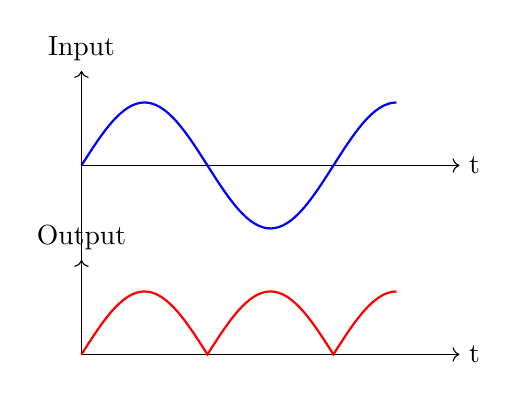
\begin{tikzpicture}[scale=0.8]
    \draw[->] (0,0) -- (6,0) node[right] {t};
    \draw[->] (0,-1.5) -- (0,1.5) node[above] {Input};
    \draw[thick, blue] (0,0) sin (1,1) cos (2,0) sin (3,-1) cos (4,0) sin (5,1);
    
    \begin{scope}[yshift=-3cm]
        \draw[->] (0,0) -- (6,0) node[right] {t};
        \draw[->] (0,0) -- (0,1.5) node[above] {Output};
        \draw[thick, red] (0,0) sin (1,1) cos (2,0) sin (3,1) cos (4,0) sin (5,1);
    \end{scope}
\end{tikzpicture}
\caption{Input AC and Output Pulsating DC}
\end{figure}

\paragraph{Mnemonic:}
\emph{Center Tap = 2 Diodes, Both Halves Conduct.}

\subsection*{OR}

\subsection{Question 2(a) [3 marks]}
\textbf{Explain concept of capacitors.}

\subsubsection{Solution}
A **capacitor** is a passive component that stores electrical energy in an electric field.

\paragraph{Key Points:}
\begin{itemize}
    \item **Construction:** Two conductive plates separated by an insulator (dielectric).
    \item **Formula:** \(C = \frac{Q}{V}\) where C is capacitance (Farads), Q is charge, V is voltage.
    \item **Function:** Blocks DC, passes AC characteristics. Used filtering, coupling, and timing circuits.
    \item **Energy Stored:** \(E = \frac{1}{2} C V^2\).
\end{itemize}

\paragraph{Mnemonic:}
\emph{Capacitor = Storage Tank for Charge.}

\subsection{Question 2(b) [4 marks]}
\textbf{Calculate value of resistor and tolerance for following color bands on resistor:}
\begin{enumerate}
    \item Brown, Green, yellow, gold
    \item Grey, blue, brown
\end{enumerate}

\subsubsection{Solution}

\paragraph{1. Brown, Green, Yellow, Gold:}
\begin{itemize}
    \item Brown (1), Green (5) \(\rightarrow\) 15
    \item Yellow (Multiple \(10^4\))
    \item Gold (Tolerance \(\pm 5\%\))
    \item **Value:** \(15 \times 10^4\,\Omega = 150,000\,\Omega = 150\,k\Omega \pm 5\%\)
\end{itemize}

\paragraph{2. Grey, Blue, Brown:}
\begin{itemize}
    \item Grey (8), Blue (6) \(\rightarrow\) 86
    \item Brown (Multiplier \(10^1\))
    \item No 4th band (Assume \(\pm 20\%\))
    \item **Value:** \(86 \times 10^1\,\Omega = 860\,\Omega \pm 20\%\)
\end{itemize}

\paragraph{Mnemonic:}
\emph{Band1-Digit, Band2-Digit, Band3-Multiplier, Band4-Tolerance.}

\subsection{Question 2(c) [7 marks]}
\textbf{Explain working of Full wave bridge rectifier with circuit diagram and wave form.}

\subsubsection{Solution}

\paragraph{Circuit Diagram:}
\begin{figure}[H]
\centering
\begin{circuitikz}[scale=1.0]
    \draw (0,2) to[sV, l=\(V_{in}\)] (0,-2);
    % Bridge
    \draw (3,0) to[D, l=\(D_1\)] (4.5, 1.5);
    \draw (4.5, 1.5) to[D, l=\(D_2\)] (6,0);
    \draw (4.5, -1.5) to[D, l=\(D_3\)] (3,0);
    \draw (6,0) to[D, l=\(D_4\)] (4.5, -1.5);
    
    % Connections
    \draw (0,2) -- (4.5,2) -- (4.5,1.5);
    \draw (0,-2) -- (4.5,-2) -- (4.5,-1.5);
    
    % Load
    \draw (3,0) -- (3, -3) -- (5.5, -3);
    \draw (6,0) -- (6, -0.5) to[R, l=\(R_L\)] (6, -2.5) -- (5.5, -2.5) -- (5.5, -3) node[ground]{};
    
    \node at (6.5, -1.5) {\(V_{out}\)};
\end{circuitikz}
\caption{Full Wave Bridge Rectifier}
\end{figure}

\paragraph{Working:}
\begin{itemize}
    \item Uses 4 diodes (\(D_1-D_4\)) in a bridge topology.
    \item **Positive Half:** \(D_2\) and \(D_4\) conduct (Forward), \(D_1\) and \(D_3\) OFF. Path: Source \(\rightarrow D_2 \rightarrow Load \rightarrow D_4 \rightarrow\) Return.
    \item **Negative Half:** \(D_1\) and \(D_3\) conduct, \(D_2\) and \(D_4\) OFF. Path: Source \(\rightarrow D_3 \rightarrow Load \rightarrow D_1 \rightarrow\) Return.
    \item Output is pulsating DC. Efficiency is 81.2%. No center tap transformer needed.
\end{itemize}

\paragraph{Waveforms:}
Same as Center Tap Rectifier (Full Wave).

\paragraph{Mnemonic:}
\emph{Bridge = 4 Diodes, High Efficiency, No Center Tap.}

% ========================================
% QUESTION 3
% ========================================
\section{Question 3}

\subsection{Question 3(a) [3 marks]}
\textbf{Explain Light dependent resistor (LDR).}

\subsubsection{Solution}
**LDR (Light Dependent Resistor)**, also known as a photoresistor, is a component whose resistance varies with light intensity.

\paragraph{Key Points:}
\begin{itemize}
    \item **Principle:** Photoconductivity.
    \item **Operation:**
        \begin{itemize}
            \item **Dark:** High resistance (\(M\Omega\) range).
            \item **Light:** Low resistance (few hundred \(\Omega\)).
        \end{itemize}
    \item **Material:** Cadmium Sulfide (CdS).
    \item **Application:** Street lights, Camera shutter control.
\end{itemize}

\paragraph{Mnemonic:}
\emph{LDR: Light Up -> Resistance Down.}

\subsection{Question 3(b) [4 marks]}
\textbf{Explain half wave rectifier circuit with wave form.}

\subsubsection{Solution}

\paragraph{Circuit Diagram:}
\begin{figure}[H]
\centering
\begin{circuitikz}[scale=1.0]
    \draw (0,0) to[sV, l=\(V_{in}\)] (0,2) -- (2,2) to[D, l=D] (4,2) to[R, l=\(R_L\)] (4,0) -- (0,0);
    \node at (5,1) {\(V_{out}\)};
\end{circuitikz}
\end{figure}

\paragraph{Explanation:}
\begin{itemize}
    \item **Positive Half:** Anode positive wrt Cathode \(\rightarrow\) Diode ON \(\rightarrow\) Current flows.
    \item **Negative Half:** Anode negative wrt Cathode \(\rightarrow\) Diode OFF \(\rightarrow\) No current.
    \item **Result:** Only positive half cycles appear at output.
    \item **Efficiency:** Max 40.6\%.
\end{itemize}

\paragraph{Waveform:}
Output exists only for \(0-\pi\), \(2\pi-3\pi\), etc. Zero for \(\pi-2\pi\).

\paragraph{Mnemonic:}
\emph{Half Wave = One Diode, 50\% (approx) loss.}

\subsection{Question 3(c) [7 marks]}
\textbf{List different types of clipper circuits and draw any two types of clipper circuits with its wave forms.}

\subsubsection{Solution}

\paragraph{List of Clipper Circuits:}
\begin{enumerate}
    \item Positive Clipper (Series/Shunt)
    \item Negative Clipper (Series/Shunt)
    \item Biased Clipper (Positive/Negative)
    \item Combination Clipper
\end{enumerate}

\paragraph{1. Positive Shunt Clipper:}
Removes positive half of the waveform.
\begin{figure}[H]
\centering
\begin{circuitikz}[scale=0.8]
    \draw (0,0) to[sV] (0,2) to[R] (2,2) -- (4,2);
    \draw (2,2) to[D, l=D] (2,0);
    \draw (0,0) -- (4,0);
    \node[right] at (4,1) {Only Negative Half remains};
\end{circuitikz}
\end{figure}
**Waveform:** Output is zero during positive cycle (Diode Short), follows input during negative (Diode Open).

\paragraph{2. Negative Series Clipper:}
Removes negative half.
\begin{figure}[H]
\centering
\begin{circuitikz}[scale=0.8]
    \draw (0,0) to[sV] (0,2) to[D, l=D] (2,2) to[R] (2,0) -- (0,0);
\end{circuitikz}
\end{figure}
**Waveform:** Output exists only for positive cycle.

\paragraph{Mnemonic:}
\emph{Clipper: Scissors applied to Waveform (Clips off parts).}

\subsection*{OR}

\subsection{Question 3(a) [3 marks]}
\textbf{Explain self and mutual inductance in brief.}

\subsubsection{Solution}

\paragraph{Definitions:}
\begin{description}
    \item[Self Inductance (L):] The property of a coil to oppose any change in current flowing through **itself** by inducing an EMF (\(V = -L \frac{di}{dt}\)).
    \item[Mutual Inductance (M):] The property where a changing current in one coil induces an EMF in a **neighboring** coil.
\end{description}

\paragraph{Mnemonic:}
\emph{Self = Me (My current opposes me). Mutual = Us (Your current affects me).}

\subsection{Question 3(b) [4 marks]}
\textbf{Explain the following terms in brief. (1) Ripple factor (2) Ripple frequency}

\subsubsection{Solution}

\paragraph{Definitions:}
\begin{description}
    \item[Ripple Factor (\(\gamma\)):] The ratio of RMS value of AC component to the DC component in the output working.
    \[ \gamma = \frac{V_{ac(rms)}}{V_{dc}} \]
    Indicates how smooth the DC output is. Lower is better.
    
    \item[Ripple Frequency (\(f_r\)):] The frequency of the AC component (ripple) present in the DC output.
    \begin{itemize}
        \item Half Wave: \(f_r = f_{in}\) (50Hz)
        \item Full Wave: \(f_r = 2f_{in}\) (100Hz)
    \end{itemize}
\end{description}

\paragraph{Mnemonic:}
\emph{Factor = Ratio (AC/DC). Frequency = Rate of pulses.}

\subsection{Question 3(c) [7 marks]}
\textbf{List different types of clamper circuits and draw any two types of clamper circuits with its wave forms.}

\subsubsection{Solution}
Circuit that shifts the DC level of a signal without changing its shape.

\paragraph{Types:}
\begin{enumerate}
    \item Positive Clamper
    \item Negative Clamper
    \item Biased Clamper
\end{enumerate}

\paragraph{1. Positive Clamper:}
Shifts waveform UP (Negative peak connects to zero/bias).
\begin{figure}[H]
\centering
\begin{circuitikz}[scale=0.8]
    \draw (0,0) to[sV] (0,2) to[C] (2,2) to[D, l=D, invert] (2,0) -- (0,0);
    \draw (2,2) -- (3,2) to[R] (3,0) -- (2,0);
\end{circuitikz}
\end{figure}
**Waveform:** Input (ex: -5V to +5V) becomes Output (0V to +10V).

\paragraph{2. Negative Clamper:}
Shifts waveform DOWN.
\begin{figure}[H]
\centering
\begin{circuitikz}[scale=0.8]
    \draw (0,0) to[sV] (0,2) to[C] (2,2) to[D, l=D] (2,0) -- (0,0);
    \draw (2,2) -- (3,2) to[R] (3,0) -- (2,0);
\end{circuitikz}
\end{figure}
**Waveform:** Input (-5V to +5V) becomes Output (-10V to 0V).

\paragraph{Mnemonic:}
\emph{Clamper: Elevator (Lifts signal Up or Down).}

% ========================================
% QUESTION 4
% ========================================
\section{Question 4}

\subsection{Question 4(a) [3 marks]}
\textbf{Draw Symbols of Zener diode, LED, and Varactor diode.}

\subsubsection{Solution}

\paragraph{Symbols:}
\begin{figure}[H]
\centering
\begin{circuitikz}[scale=1.2]
    % Zener
    \draw (0,0) to[zD, l=Zener] (0,2);
    % LED
    \draw (3,0) to[leDo, l=LED] (3,2);
    % Varactor
    \draw (6,0) to[VCo, l=Varactor] (6,2);
\end{circuitikz}
\caption{Diode Symbols}
\end{figure}

\paragraph{Mnemonic:}
\emph{Zener: Z shape. LED: Arrows Out (Light Emitting). Varactor: Capacitor symbol + Diode.}

\subsection{Question 4(b) [4 marks]}
\textbf{Explain Photodiode.}

\subsubsection{Solution}
A **Photodiode** is a PN junction diode designed to operate in **reverse bias**. It converts light energy into electrical current.

\paragraph{Working:}
\begin{itemize}
    \item When light falls on the junction, electron-hole pairs are generated.
    \item In reverse bias, these carriers are swept across the junction, creating a reverse current (\(I_{\lambda}\)) proportional to light intensity.
    \item Dark current flows when no light is present (very small).
\end{itemize}

\paragraph{Mnemonic:}
\emph{Photo = Light, Reverse Bias, Light In -> Current Flow.}

\subsection{Question 4(c) [7 marks]}
\textbf{Explain construction, characteristics and working of Zener diode.}

\subsubsection{Solution}

\paragraph{Construction:}
\begin{itemize}
    \item Heavily doped P-N junction diode.
    \item Thin depletion layer.
    \item Designed to operate in breakdown region without damage.
\end{itemize}

\paragraph{Working:}
\begin{itemize}
    \item **Forward Bias:** Acts like a normal diode.
    \item **Reverse Bias:**
        \begin{itemize}
            \item Until breakdown voltage (\(V_z\)), very little current flows.
            \item At \(V_z\), current increases sharply due to Zener Effect (tunneling) or Avalanche Effect.
            \item Voltage remains constant across it despite change in current.
        \end{itemize}
\end{itemize}

\paragraph{Characteristics (V-I Curve):}
\begin{figure}[H]
\centering
\begin{tikzpicture}[scale=0.7]
    \draw[->] (-4,0) -- (2,0) node[right]{V};
    \draw[->] (0,-3) -- (0,3) node[above]{I};
    \draw[thick, blue] (0,0) -- (0.7,0) -- (0.7,2.5); % Forward
    \draw[thick, blue] (0,0) -- (-2.5,0) -- (-2.5,-2.5); % Reverse Breakdown
    \node at (-2.5,-3) {\(V_z\)};
    \node at (1.5,1) {Forward};
    \node at (-1,-1) {Reverse};
\end{tikzpicture}
\caption{Zener Characteristics}
\end{figure}

\paragraph{Mnemonic:}
\emph{Zener = Reverse Breakdown, Voltage Stabilizer.}

\subsection*{OR}

\subsection{Question 4(a) [3 marks]}
\textbf{List applications of LED and Varactor diode.}

\subsubsection{Solution}

\paragraph{Applications:}
\begin{description}
    \item[LED (Light Emitting Diode):]
        \begin{itemize}
            \item Indicators (Power on/off).
            \item Displays (7-segment, Screens).
            \item Lighting (Traffic lights, Homes).
            \item Optical Communication (Fiber optics).
        \end{itemize}
    \item[Varactor Diode:]
        \begin{itemize}
            \item Tuning circuits (Radio/TV tuners).
            \item Frequency multipliers.
            \item Voltage Controlled Oscillators (VCO).
            \item Filters (Tunable).
        \end{itemize}
\end{description}

\paragraph{Mnemonic:}
\emph{LED = Light/Display. Varactor = Tuning (Variable Reactor).}

\subsection{Question 4(b) [4 marks]}
\textbf{Explain Zener diode as a voltage regulator.}

\subsubsection{Solution}

\paragraph{Circuit Diagram:}
\begin{figure}[H]
\centering
\begin{circuitikz}[scale=1.0]
    \draw (0,0) to[V, l=\(V_{in}\)] (0,3);
    \draw (0,3) to[R, l=\(R_s\)] (3,3);
    \draw (3,3) to[zD, l=\(V_z\)] (3,0);
    \draw (3,3) -- (5,3) to[R, l=\(R_L\)] (5,0) -- (0,0);
    \node at (5.5, 1.5) {\(V_{out} = V_z\)};
\end{circuitikz}
\caption{Zener Voltage Regulator}
\end{figure}

\paragraph{Operation:}
\begin{itemize}
    \item Zener is connected in **parallel** (shunt) with load, in **reverse bias**.
    \item If \(V_{in}\) increases, Zener current (\(I_z\)) increases, increasing drop across series resistor (\(R_s\)).
    \item \(V_{out}\) remains clamped at \(V_z\).
    \item Effectively absorbs excess current to keep voltage constant.
\end{itemize}

\paragraph{Mnemonic:}
\emph{Shunt Regulator: Zener eats the extra current to save voltage.}

\subsection{Question 4(c) [7 marks]}
\textbf{Explain construction, characteristics and working of Varactor diode.}

\subsubsection{Solution}

\paragraph{Construction:}
\begin{itemize}
    \item A P-N junction diode optimized for **variable capacitance**.
    \item Operates in **reverse bias**.
    \item Depletion layer acts as dielectric, P and N regions act as plates.
\end{itemize}

\paragraph{Working:}
\begin{itemize}
    \item Reverse voltage determines width of depletion layer (\(W\)).
    \item Capacitance \(C = \frac{\epsilon A}{W}\).
    \item Higher Reverse Voltage \(\rightarrow\) Wider Depletion Layer (\(W \uparrow\)) \(\rightarrow\) Lower Capacitance (\(C \downarrow\)).
    \item Used as a voltage-controlled capacitor.
\end{itemize}

\paragraph{Characteristics:}
Graph of Capacitance (C) vs Reverse Voltage (\(V_R\)) shows inverse relationship. C decreases as \(V_R\) increases.

\paragraph{Mnemonic:}
\emph{Varactor = Variable Capacitor. Voltage Up -> Cap Down.}

% ========================================
% QUESTION 5
% ========================================
\section{Question 5}

\subsection{Question 5(a) [3 marks]}
\textbf{Explain transistor as a switch.}

\subsubsection{Solution}
A transistor (BJT) works as a switch by operating in Cut-off and Saturation regions.

\begin{itemize}
    \item **OFF State (Open Switch):** Works in **Cut-off** region. Base current \(I_B = 0\), so \(I_C = 0\). \(V_{CE} = V_{CC}\).
    \item **ON State (Closed Switch):** Works in **Saturation** region. Base current is high. \(V_{CE} \approx 0\) (Saturation voltage). Max current flows.
\end{itemize}

\paragraph{Mnemonic:}
\emph{Cutoff = OPEN. Saturation = CLOSED.}

\subsection{Question 5(b) [4 marks]}
\textbf{Draw Common Emitter (CE) configuration of NPN transistors and its input characteristics.}

\subsubsection{Solution}
\begin{paragraph}{Circuit Diagram:}
\begin{figure}[H]
\centering
\begin{circuitikz}[scale=0.8]
    \draw (0,0) node[npn](Q){} ;
    \draw (Q.E) node[ground]{}; % Common Emitter
    \draw (Q.B) -- ++(-1,0) node[left]{Input};
    \draw (Q.C) -- ++(1,0) node[right]{Output};
\end{circuitikz}
\end{figure}
\end{paragraph}

\begin{paragraph}{Input Characteristics:}
Graph of Base Current (\(I_B\)) vs Base-Emitter Voltage (\(V_{BE}\)) at constant \(V_{CE}\). 
Similar to a forward-biased diode curve. Current rises effectively after \(V_{BE} > 0.7V\) (Si).
\end{paragraph}

\paragraph{Mnemonic:}
\emph{Input Char = Diode Curve (Ib vs Vbe).}

\subsection{Question 5(c) [7 marks]}
\textbf{Draw symbol and construction of NPN Transistor and explain its working.}

\subsubsection{Solution}

\paragraph{Structure:}
\begin{itemize}
    \item **NPN:** P-type layer sandwiched between two N-type layers.
    \item **Terminals:** Emitter (Heavily doped), Base (Lightly doped, thin), Collector (Moderately doped, large area).
\end{itemize}

\paragraph{Symbol:}
\begin{figure}[H]
\centering
\begin{circuitikz}
    \draw (0,0) node[npn, l=NPN](Q){};
\end{circuitikz}
\caption{NPN Symbol (Arrow Out)}
\end{figure}

\paragraph{Working (Active Mode):}
\begin{itemize}
    \item Emitter-Base junction is **Forward Biased**. Collector-Base is **Reverse Biased**.
    \item Electrons injected from Emitter to Base.
    \item Since Base is thin, most electrons (\(>95\%\)) cross Base and are swept into Collector by high potential.
    \item \(I_E = I_B + I_C\). Small \(I_B\) controls large \(I_C\).
\end{itemize}

\paragraph{Mnemonic:}
\emph{NPN: Not Pointing In (Arrow points out). Emitter Emits, Base Controls, Collector Collects.}

\subsection*{OR}

\subsection{Question 5(a) [3 marks]}
\textbf{Compare CB, CE and CC configuration of transistor.}

\subsubsection{Solution}

\begin{table}[H]
\centering
\begin{tabular}{|l|l|l|l|}
\hline
Parameter & Common Base (CB) & Common Emitter (CE) & Common Collector (CC) \\ \hline
Input Res & Low & Medium & High \\ \hline
Output Res & High & Medium & Low \\ \hline
Current Gain & Low (\(<1\)) & High (\(\beta\)) & High (\(\gamma\)) \\ \hline
Voltage Gain & High & High & Low (\(<1\)) \\ \hline
Phase Shift & 0 & 180 degrees & 0 \\ \hline
Used as & HF Apps & Audio Amp & Impedance Matching \\ \hline
\end{tabular}
\end{table}

\paragraph{Mnemonic:}
\emph{CE is Best for Power/Audio (Universal). CC is Buffer. CB is HF.}

\subsection{Question 5(b) [4 marks]}
\textbf{Explain transistor as a single stage common emitter amplifier.}

\subsubsection{Solution}

\paragraph{Circuit:}
Uses an NPN transistor in CE mode with voltage divider biasing.
\begin{itemize}
    \item **Biasing:** \(R_1, R_2\) provide stable bias to Base.
    \item **Coupling Caps:** \(C_{in}, C_{out}\) block DC.
    \item **Bypass Cap:** \(C_E\) across \(R_E\) to prevent AC gain reduction.
\end{itemize}

\paragraph{Working:}
\begin{itemize}
    \item Small AC signal at Base fluctuates base current \(I_B\).
    \item This causes large fluctuation in \(I_C\) (\(\beta\) times larger).
    \item Varying \(I_C\) flows through \(R_C\) to produce amplified voltage swing at output.
    \item Output is \(180^\circ\) phase shifted.
\end{itemize}

\paragraph{Mnemonic:}
\emph{CE Amp: Small Signal In -> Large Inverted Signal Out.}

\subsection{Question 5(c) [7 marks]}
\textbf{Explain common base (CB) configuration of NPN transistors with its input-output characteristics.}

\subsubsection{Solution}

\paragraph{Circuit:}
Base is common to both input and output.
\begin{itemize}
    \item Input applied between Emitter and Base.
    \item Output taken between Collector and Base.
\end{itemize}

\paragraph{Characteristics:}
\begin{description}
    \item[Input (\(I_E\) vs \(V_{EB}\)):] Similar to diode. \(I_E\) increases rapidly for small \(V_{EB}\).
    \item[Output (\(I_C\) vs \(V_{CB}\)):] Almost horizontal lines. \(I_C\) depends mostly on \(I_E\), independent of \(V_{CB}\) (Active region).
    \item[Current Gain (\(\alpha\)):] Ratio \(I_C / I_E\). Always slight less than 1 (0.95 to 0.99).
\end{description}

\paragraph{Mnemonic:}
\emph{CB: Current Gain < 1, Voltage Gain High.}

\end{document}
